%!TEX root = ms.tex
\section{Justification of hdf and AICc}
\label{sec:justification_aicc_hdf}

In this section, we provide justifications for hdf and AICc as a heuristic degrees of freedom and a selection rule for BS, respectively, when the predictors $X$ are orthogonal.

\subsection{The heuristic degrees of freedom}
\label{sec:justification_hdf}

We provide a theoretical justification for hdf in a restricted scenario where $X$ is orthogonal and the true model is null. We further give numerical justification for a general true model, and demonstrate the use of hdf in model selection for BS. 

\subsubsection{Theoretical justification of hdf under a null true model}
Assume $\mu=0$, with $X$ still being orthogonal. In such a restricted scenario, df$_C(k)$ (edf of BS for subset size $k$) has an analytical expression, which allows us to provide some theoretical justification for hdf$(k)$. We start by introducing notation, and present the main result in Theorem \ref{thm:hdf_ydf_representation} and its Corollary. The detailed proofs are given in the Supplemental Material Section \ref{sec:proof_hdf_ydf}.

Denote $\tilde{X}_{(i)}$ as the $i$-th largest order statistic in an i.i.d sample of size $p$ from a $\chi^2_1$ distribution. \citet{Ye1998} showed that
\begin{equation*}
\text{df}_C(k) = E\left( \sum_{i=1}^{k} \tilde{X}_{(i)} \right).
\end{equation*}
Let $\tilde{H}(s) = -\tilde{Q}(1-s)$ where $\tilde{Q}$ is the quantile function of a $\chi_1^2$ distribution, and $s\in (0,1)$. For $0\le s \le t \le 1$, the truncated variance function is defined as
\begin{equation*}
\tilde{\sigma}^2(s,t) = \int_{s}^{t} \int_{s}^{t} (u \wedge v -uv) d \tilde{H}(u) d \tilde{H}(v),
\end{equation*}
where $u \wedge v =\min(u,v)$. Denote $\tilde{Y}_p = \tilde{\sigma}_p^{-1}(\sum_{i=1}^k \tilde{X}_{(i)} - \tilde{\mu}_p)$, where
\begin{equation*}
\tilde{\sigma}_p = \sqrt{p} \cdot \tilde{\sigma}(1/p,k/p),
\end{equation*}
and
\begin{equation*}
\tilde{\mu}_p = -p \int_{1/p}^{k/p} \tilde{H}(u) du - \tilde{H}\left(\frac{1}{p}\right).
\end{equation*}

\begin{restatable}{theorem}{dfasy}
	\label{thm:hdf_ydf_representation}
	Assume $X$ is orthogonal and the true model is null ($\mu=0$). As $p\rightarrow  \infty$,  $k\rightarrow  \infty$ with $k=\left \lfloor{px}\right \rfloor$, we have
	\begin{equation}
	\label{eq:hdf_ydf_yp_representation}
	\frac{1}{2p} \text{hdf}(k) = \frac{1}{2p}\text{df}_C(k) - \frac{\tilde{\sigma}_p}{2p}E(\tilde{Y}_p) + O\left(\frac{\log(p)}{p} \right),
	\end{equation}
	where $x \in (0,1)$ is a constant and $\left \lfloor{\cdot}\right \rfloor$ denotes the greatest integer function.
\end{restatable}

\begin{restatable}{corollary}{dfasycorollary}
	\label{thm:hdf_ydf_corollary}
	If $\limsup |E(\tilde{Y}_p)| < \infty$ , we further have
	\begin{equation}
	\label{eq:main_corollary}
	\frac{\text{df}_C(k)}{\text{hdf}(k)} \rightarrow 1.
	\end{equation}
\end{restatable}
\noindent\textbf{Remark:} If $\tilde{Y}_p$ is uniformly integrable, then $E(\tilde{Y}_p) \rightarrow 0$, and hence the result of Corollary \ref{thm:hdf_ydf_corollary} holds.

It can be seen that Corollary \ref{thm:hdf_ydf_corollary} holds given the assumptions, since both hdf$(k)$ and df$_C(k)$ diverge while $E(\tilde{Y}_p)$ and the remainder term remain bounded. The Corollary suggests that for large $k$ and large $p$, the ratio of df$_C(k)$ to hdf$(k)$ will be close to $1$. We next explore empirically the relative behavior of the two dfs for a fixed $p$ with an increasing $k$. 

\subsubsection{Numerical justification of hdf}
Figure \ref{fig:dfc_dflambda} shows the comparison of hdf and edf via simulations. We fit BS on $1000$ realizations of the response generated after fixing $X$. The edf is calculated based on definition \eqref{eq:edf} using the sample covariances, while hdf is given by Algorithm \ref{alg:hdf}. We see that in the null case, using hdf to approximate edf becomes more accurate as $k$ approaches $p$, providing a finite-sample justification of Corollary \ref{thm:hdf_ydf_corollary}. 

In addition to the null model, we consider a sparse model (Orth-Sparse-Ex1) with $p_0=6$ true predictors (those with non-zero coefficients), and a dense model (Orth-Dense) where all predictors have non-zero coefficients. Similarly to the null case, we see that hdf approaches edf as $k$ gets close to $p$, i.e. the statement of Corollary \ref{thm:hdf_ydf_corollary} holds in these scenarios as well. Furthermore, we see that hdf generally approximates edf well, where the difference is more pronounced when BS underfits, e.g. a sparse model with high SNR and $k<p_0=6$ or a dense model with high SNR with $k<p=14$. Clearly, underfitting causes the problem, particularly when what is left out is important, such as in a high SNR case.   


% \ref{fig:dfc_dflambda}
\begin{figure}[!ht]
	\centering
	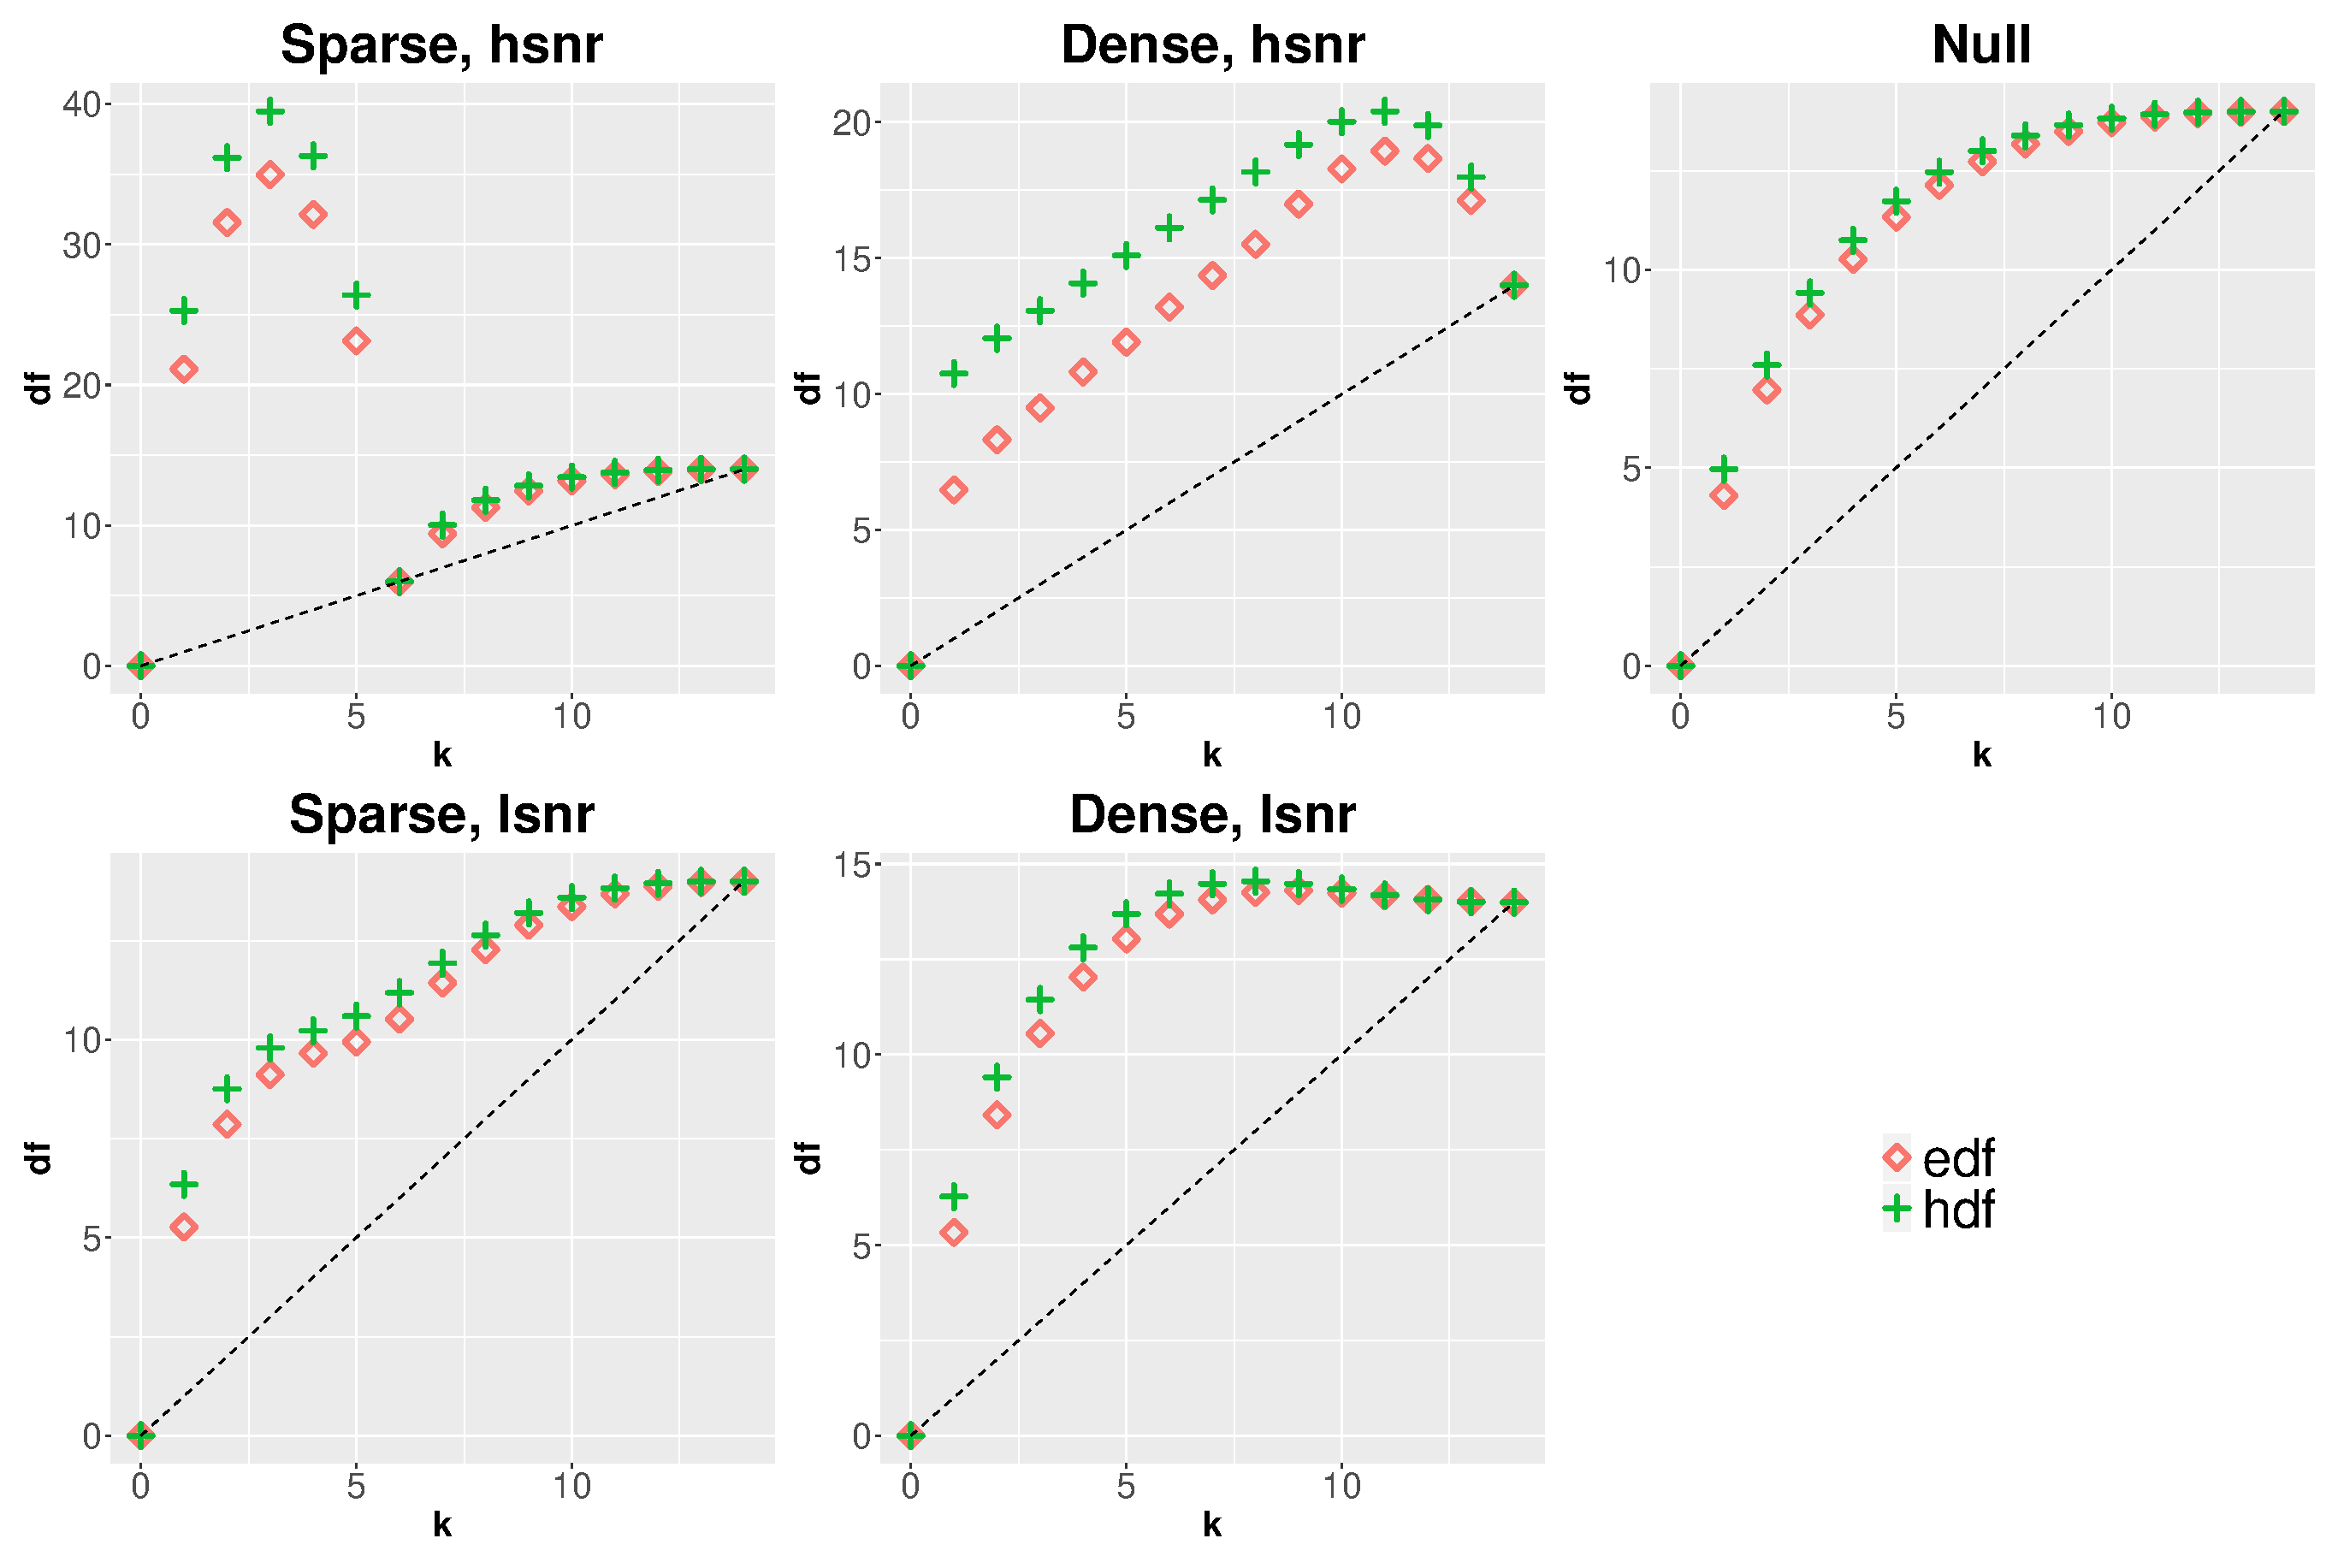
\includegraphics[width=0.9\textwidth]{figures/hdf_edf_bs.eps}
	\caption{hdf$(k)$ and df$_C(k)$ (edf of constrained BS). The black dashed line is the 45-degree line. Here $X$ is orthogonal with $n=200$ and $p=14$. Three types of the true model and two SNR are considered. We assume knowledge of $\mu$ and $\sigma$.}
	\label{fig:dfc_dflambda}
\end{figure}



\subsubsection{\texorpdfstring{C$_p$}{Lg}-hdf as a feasible implementation of \texorpdfstring{C$_p$}{Lg}-edf }
\label{sec:cp_edf_hdf}
We have shown that hdf generally approximates edf well, and agrees with edf in some situations as $k$ approaches $p$. By replacing edf with hdf in \eqref{eq:cp_edf}, we have a feasible selection rule C$_p$-hdf. Figure \ref{fig:cp_edf_hdf} compares the averages of C$_p$-edf and C$_p$-hdf over $1000$ replications. Similarly to the comparison of the degrees of freedom values, we see C$_p$-hdf agrees with C$_p$-edf on average as $k$ approaches $p$. Even at the places where we see differences between the degrees of freedom values, e.g. a sparse true model with high SNR and $k<p_0=6$, the differences are compensated by the model fit and we see C$_p$-hdf is very close to C$_p$-edf. As we discussed in Section \ref{sec:optimism}, for any general fitting procedure including BS, C$_p$-edf provides an unbiased estimator of the expected prediction error where the error measure $\Theta$ is the squared error (SE), i.e. $E(\text{C}_p\text{-edf}) = E(\text{Err}_{\text{SE}})$. Therefore, by using the sample average to represent the population mean, Figure \ref{fig:cp_edf_hdf} indicates that $E(\text{C}_p\text{-hdf})$ approximates $E(\text{Err}_{\text{SE}})$ well, and moreover C$_p$-hdf gives the same average selected size as C$_p$-edf in all cases, when they are applied as selection rules, supporting the use of hdf in model selection for BS under orthogonal predictors.

% \ref{fig:cp_edf_hdf} 
\begin{figure}[!ht]
	\centering
	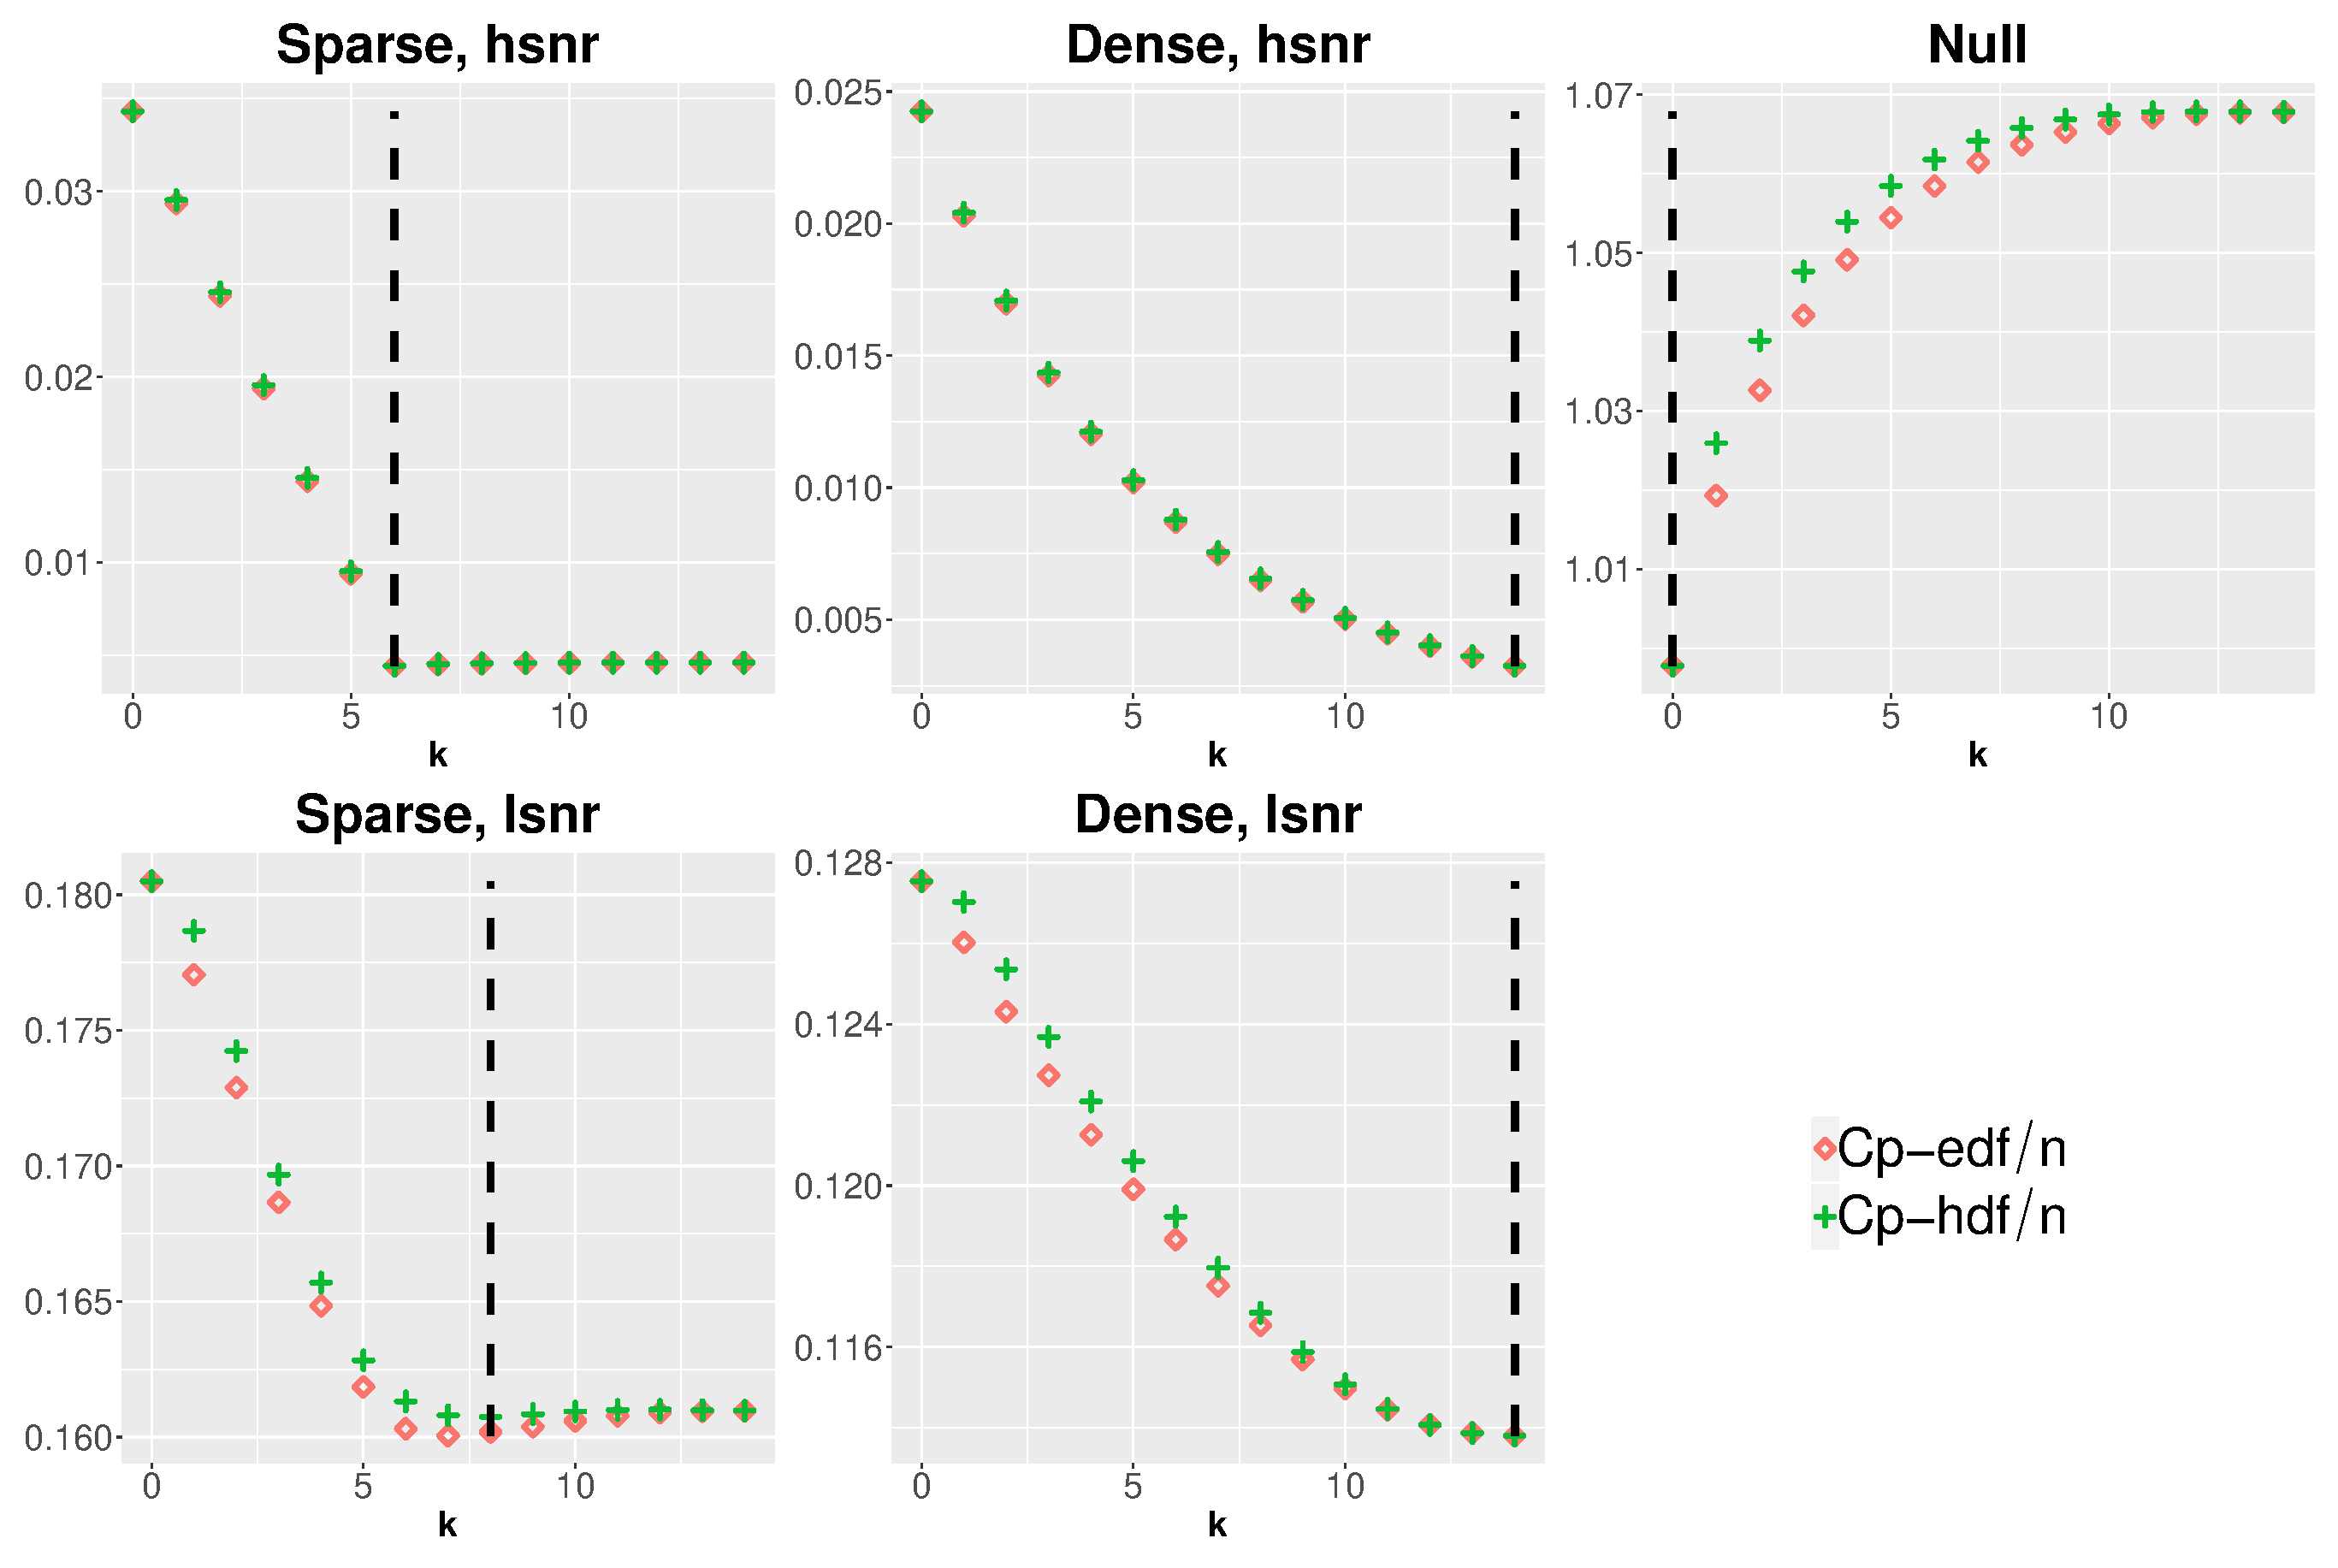
\includegraphics[width=0.9\textwidth]{figures/cp_edf_hdf_bs.eps}
	\caption{Averages of C$_p$-edf and C$_p$-hdf over $1000$ replications. Both criteria lead to the same average of the selected subset size over the $1000$ replications (rounded to the nearest integer), as denoted by the black dashed vertical lines. Other details are the same as in Figure \ref{fig:dfc_dflambda}.}
	\label{fig:cp_edf_hdf} 
\end{figure}


\subsection{A KL-based information criterion for BS}
When the error measure $\Theta$ is the deviance \eqref{eq:deviance_def}, the prediction error $\text{Err}_\text{KL}$ is the KL discrepancy. AICc-edf \eqref{eq:aicc_edf} is motivated by trying to construct an unbiased estimator of $E(\text{Err}_\text{KL})$. The expected KL-based optimism for BS is given as
\begin{equation}
E(\text{op}_\text{KL}) = E\left(n \frac{n\sigma^2+\lVert \mu-X\hat{\beta}(k) \rVert_2^2}{\lVert y-X\hat{\beta}(k)\rVert_2^2}\right) + n.
\label{eq:eop_expression}
\end{equation}
Note that \eqref{eq:eop_expression} holds for a general $X$. Augmenting $E(\text{op}_\text{KL})$ with the training error $\text{err}_{\text{KL}}$ we have $\widehat{\text{Err}}_{\text{KL}}$ according to \eqref{eq:err_eop}, where (ignoring the constant $n\log(2\pi)$ for convenience)
\begin{equation}
\text{err}_{\text{KL}} = n\log\left(\frac{\text{RSS}}{n}\right) - n,
\label{eq:err_expression}
\end{equation}
since the pre-specified model $f$ in \eqref{eq:deviance_def} follows a Gaussian distribution as assumed in \eqref{eq:truemodel_def}. The derivations of \eqref{eq:eop_expression} and \eqref{eq:err_expression} are presented in the Supplemental Material Section \ref{sec:expectedkl_bs}. 

Figure \ref{fig:eop_approx_withrss} shows the averages of AICc-edf, AICc-hdf and $\widehat{\text{Err}}_{\text{KL}}$ over $1000$ replications. By using the sample average to represent the population mean, we first see that $E(\text{AICc-edf})$ generally tracks the expected KL, $E(\text{Err}_{\text{KL}})$ reasonably well. In fact, they agree with each other in the null case and a sparse true model with high SNR. Noticeable discrepancies can be observed in a sparse true model with high SNR and $k<p_0=6$. This is the place where the set of true predictors is not entirely included in the model. The derivations of the classic AIC and AICc (both with ndf plugged in according to our notation) are based on an assumption that the true predictors are included in the model. In the situation where this assumption is violated, AICc will no longer be unbiased, and a similar conjecture can be made here for AICc-edf in the context of BS. Second, similarly to the comparison of $E(\text{C}_p\text{-edf})$ and $E(\text{C}_p\text{-hdf})$ in Section \ref{sec:cp_edf_hdf}, we see that $E(\text{AICc-hdf})$ approximates $E(\text{AICc-edf})$ well and they agree with each other as $k$ approaches $p$. 
Last and most importantly, both AICc-edf and AICc-hdf yield the same average selected size as $\widehat{\text{Err}}_{\text{KL}}$ across all scenarios, supporting the use of AICc-hdf as a selection rule for BS under orthogonal predictors.

% \ref{fig:eop_approx_withrss} 
\begin{figure}[!ht]
	\centering
	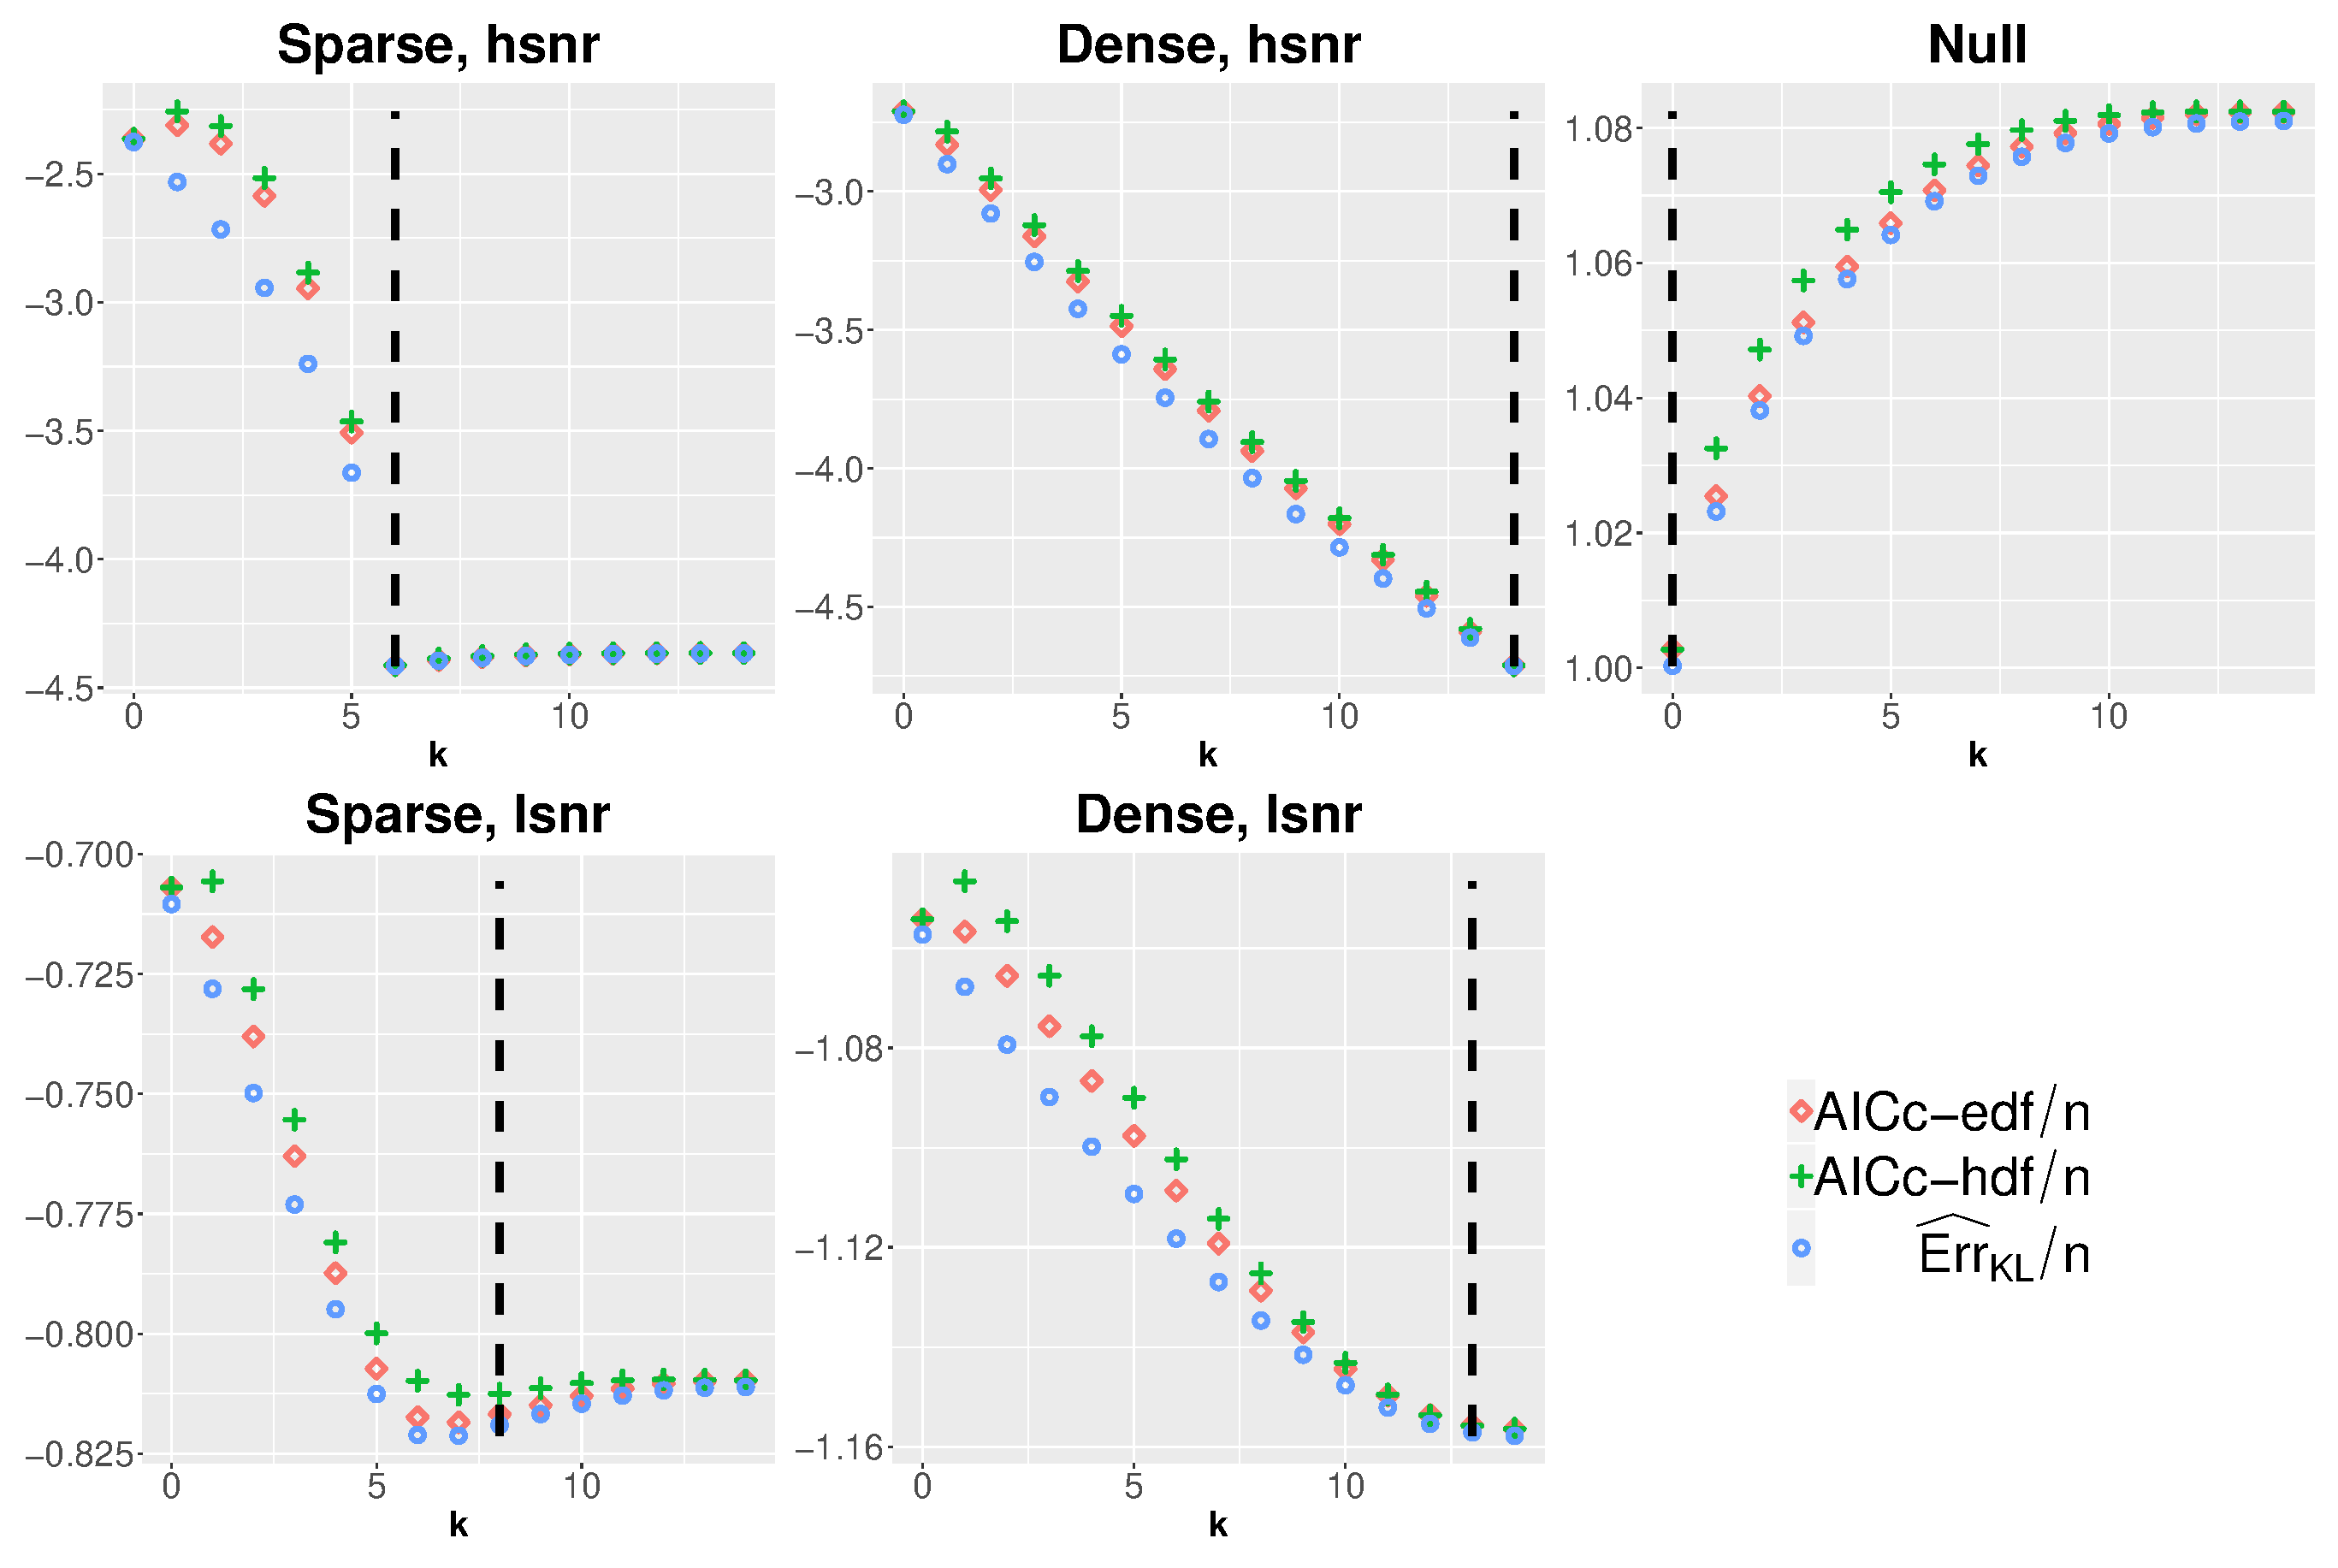
\includegraphics[width=0.9\textwidth]{figures/aicc_edf_hdf_kl_bs.eps}
	\caption{Averages of AICc-edf, AICc-hdf and $\widehat{\text{Err}}_\text{KL}$ over $1000$ replications. All three criteria lead to the same average of the selected subset size over the $1000$ replications (rounded to the nearest integer), as denoted by the black dashed vertical lines. Other details are the same as in Figure \ref{fig:dfc_dflambda}.}
	\label{fig:eop_approx_withrss} 
\end{figure}


\subsection{A discussion on the use of information criteria in LBS}
Since for orthogonal $X$ the edf of LBS has an analytical expression and LBS can recover the solution path of BS, one may ask why not just use LBS with a selection rule such as C$_p$-edf, which is well-defined for any general fitting procedure. 

\iffalse
Recall that with an orthogonal $X$, the estimated coefficients for LBS \eqref{eq:lbestsubset-setup} are $\hat{\beta}_i(\lambda)=z_i \mathbbm{1}_{(|z_{i}| \ge \sqrt{2\lambda})}$, and are $\hat{\beta}_i(k)=z_i \mathbbm{1}_{(|z_{i}| \ge |z_{(k)}|)}$ for BS \eqref{eq:bestsubset-setup}, where $z=X^T y$ and $z_{(k)}$ is the k-th largest coefficient in absolute value. Given a single realization $(X,y)$, we generate a sequence of $\lambda$ where $\sqrt{2\lambda_i} = |z_{(i)}|$ ($i=1,\cdots,p$). Between each subsequent $\lambda_i$ and $\lambda_{i+1}$, we add another $9$ equally spaced values in the log scale. 
\fi

We consider a fixed sequence of $\lambda$ and compute the LBS solutions for $1000$ realizations. The decreasing sequence of $\lambda$ starts at the smallest value $\lambda_{\text{max}}$ for which the estimated coefficient vector $\hat{\beta}$ equals zero for all of the $1000$ realizations. We then construct a sequence of $200$ values of $\lambda$ equally spaced in log scale from $\lambda_{\text{max}}$ to $\lambda_{\text{min}}$, where $\lambda_{\text{min}} = \alpha \lambda_{\text{max}}$ and $\alpha=0.001$. This procedure of generating the sequence of $\lambda$ has been discussed by \citet{Friedman2010} in the context of lasso.


We find that (see Supplemental Material Table \ref{tab:lbs_bs}) LBS is outperformed by BS in almost all scenarios based on $1000$ simulation replications. We use C$_p$-edf as the selection rule for both methods, where edf of BS (df$_C(k)$) is estimated via simulations and edf of LBS (df$_L(\lambda)$) is calculated using formulas \eqref{eq:thdf_expression} and \eqref{eq:thdf_size_expression}. We see that 1) LBS deteriorates as $p$ gets larger when SNR is low or sample size $n$ is large; and 2) increasing the sample size $n$ does not help LBS. We further compare the number of predictors given by BS and LBS for each of the $1000$ replications (see Supplemental Material Figure \ref{fig:numvar_bs_lbs}), where we consider the Orth-Sparse-Ex1 model with $n=200$ and high SNR. Under this design, LBS never selects fewer predictors than BS, and it chooses more predictors in $31.1\%$ and $37.8\%$ of all replications for $p=30$ and $p=180$, respectively. A possible explanation for this might be that df$_L(\lambda)$ characterizes the model complexity at $\lambda$ on average, but does not correctly describe the model complexity on a given realization. Given a single realization, there are an infinite number of $\lambda$ values that correspond to each distinct solution, and they lead to different values of df$_L(\lambda)$ and further result in different model complexities and different C$_p$ values. This variability in the C$_p$ values for the same solution potentially causes the selected subsets of LBS to have more variabilities than those selected subsets of BS. 




